
\chapter{Combined Results}
\label{chap:everything}

For the final chapter of the thesis, we want to provide a small insight into the effect of combining all reduction techniques that were presented. To be precise, we build several consecutive merges of an input DPA in the following order:
\begin{enumerate}
	\item Normalize $c$.
	\item Schewe merge w.r.t. $\mu_\text{skip}^{\equiv_L}$.
	\item Representative merge w.r.t. $\mu_M$.
	\item Representative merge w.r.t. $\mu_{IM}$.
	\item Representative merge w.r.t. $\mu_\text{TM}^{\equiv_L}$.
	\item Representative merge w.r.t. $\mu_\text{LSF}^{k,\equiv_L}$ for all $k$.
	\item Representative merge w.r.t. $\mu_\text{de}$.
	\item Representative merge w.r.t. $\mu_\text{PR}^\lambda$ for all classes $\lambda$ of $\equiv_L$.
\end{enumerate}

Figures \ref{fig:everything:empirical_size_hist} and \ref{fig:everything:empirical_reduct_rel} show the usual plots for efficiency and figure \ref{fig:everything:empirical_time} shows the required run time. We were actually able to reuse $\equiv_L$ after its first computation to safe a large amount of time. It anyway quickly becomes unfeasible to perform a reduction like this for growing automata.

The number of reduced states shows a satisfying result on \textsf{detspot} and \textsf{detnbaut}, with a majority of the automata witnessing a reduction of 10\% or more.


\begin{figure}
	\centering
	\begin{minipage}{0.49\textwidth}
		\includegraphics[page=6,height=.3\textheight]{../data/analysis/everything/gendet_ap1.pdf} 
		\includegraphics[page=6,height=.3\textheight]{../data/analysis/everything/detspot_ap1.pdf} 
		\includegraphics[page=6,height=.3\textheight]{../data/analysis/everything/detnbaut_ap1.pdf} 
		\caption{State reduction of different automata.}
		\label{fig:everything:empirical_size_hist}
	\end{minipage}
	\hfill
	\begin{minipage}{0.49\textwidth}
		\includegraphics[page=3,height=.3\textheight]{../data/analysis/everything/gendet_ap1.pdf} 
		\includegraphics[page=3,height=.3\textheight]{../data/analysis/everything/detspot_ap1.pdf} 
		\includegraphics[page=3,height=.3\textheight]{../data/analysis/everything/detnbaut_ap1.pdf} 
		\caption{Relative state reduction of different automata.}
		\label{fig:everything:empirical_reduct_rel}
	\end{minipage}
\end{figure}


\begin{figure}
	\centering
	\begin{minipage}{0.49\textwidth}
		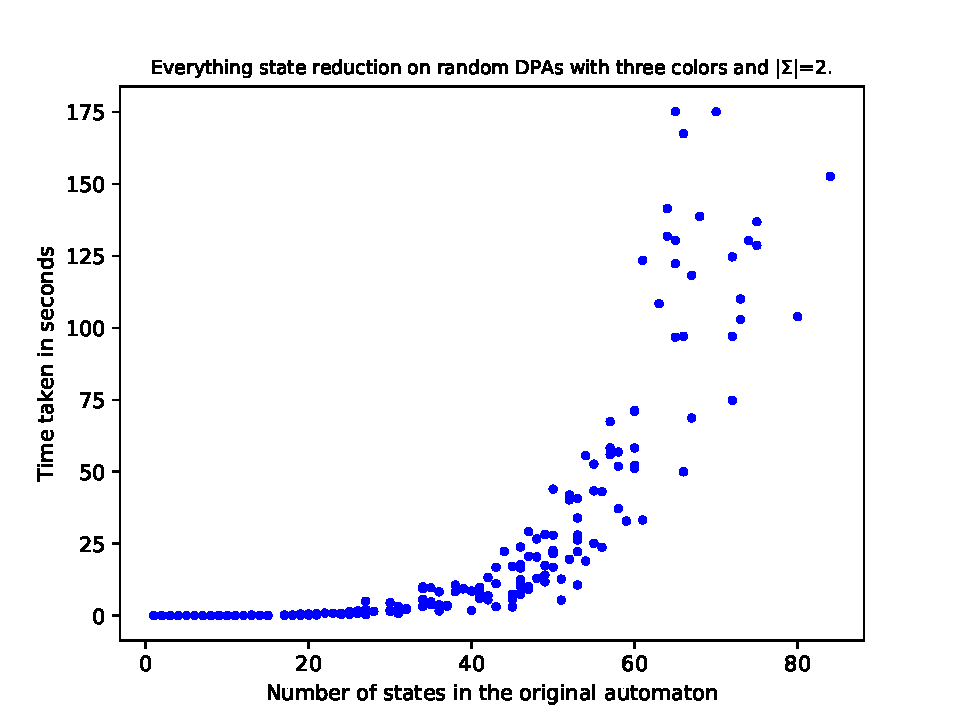
\includegraphics[page=1,height=.3\textheight]{../data/analysis/everything/gendet_ap1.pdf} 
		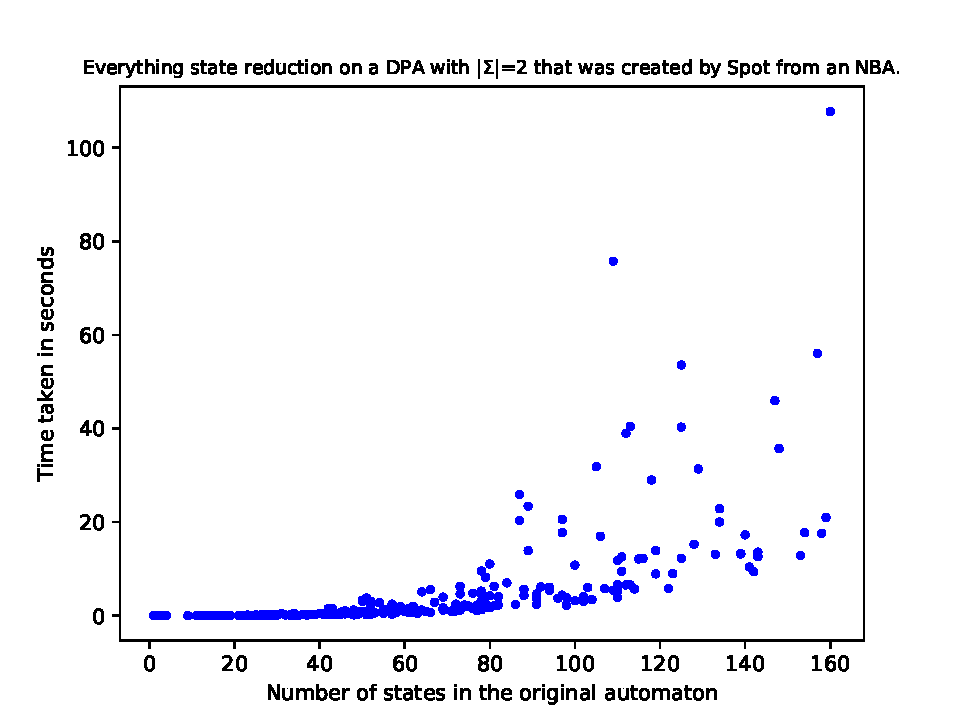
\includegraphics[page=1,height=.3\textheight]{../data/analysis/everything/detspot_ap1.pdf} 
		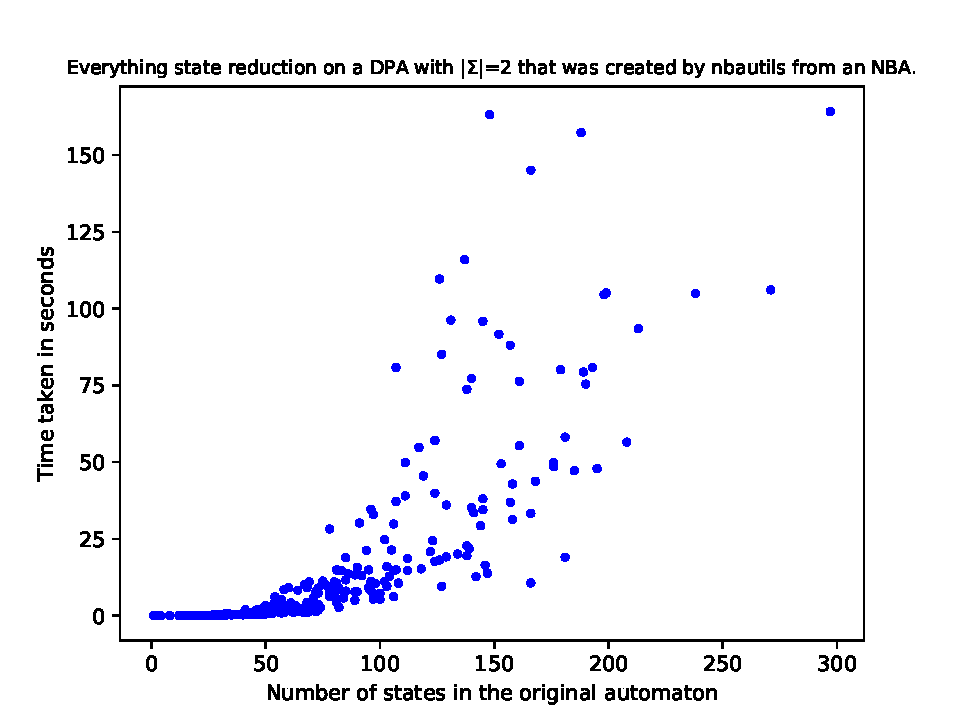
\includegraphics[page=1,height=.3\textheight]{../data/analysis/everything/detnbaut_ap1.pdf} 
		\caption{Time for state reduction of different automata.}
		\label{fig:everything:empirical_time}
	\end{minipage}
\end{figure}


We can see the effect of changing the size of $\Sigma$ in figures \ref{fig:everything:empirical_compare_time} and \ref{fig:everything:empirical_compare_reduct}. As one might expect, the run time is higher for larger alphabets; we assume that there is a linear correlation but there is not enough data to confidently support that theory.

Similarly, doubling the size of the alphabet seems to halve the efficiency of the reduction. Again, the data is not conclusive enough to support that argument with absolute certainty.




\begin{figure}
	\centering
	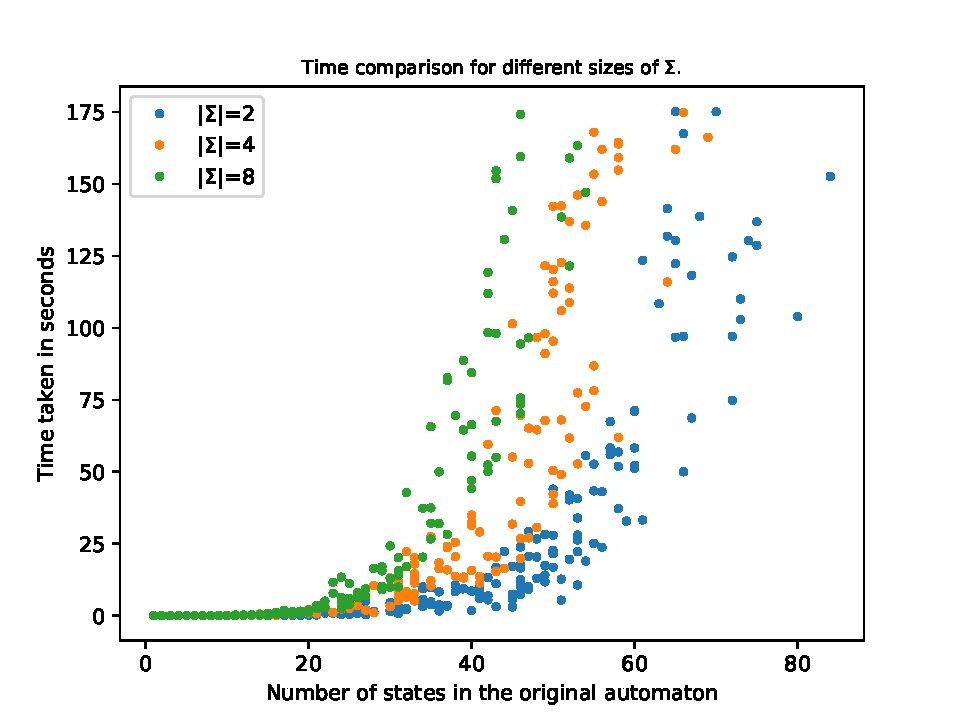
\includegraphics[page=1,height=.3\textheight]{../data/analysis/everything/ap_time_comparison.pdf} 
	\caption{Compare run time for different sizes of alphabets.}
	\label{fig:everything:empirical_compare_time}
\end{figure}


\begin{figure}
	\centering
	\includegraphics[page=2,height=.3\textheight]{../data/analysis/everything/ap_time_comparison.pdf} 
	\caption{Compare relative reduction for different sizes of alphabets.}
	\label{fig:everything:empirical_compare_reduct}
\end{figure}